% =====================================================================
%  A Training-Free Quantum-Walk Scanner for Cryptic Allosteric Sites
%  Global Quantum + AI Challenge 2026 - Cleveland Clinic
%  Phase I Concept Proposal
%
%  Compile with:  pdflatex main.tex   (twice, for references)
% =====================================================================
\documentclass[10pt,a4paper]{article}

\usepackage[T1]{fontenc}
\usepackage[utf8]{inputenc}
\usepackage{mathptmx}   % Times-like serif; swap for lmodern/newtxtext if available
\usepackage{microtype}
\usepackage{changepage}
\usepackage{multicol}
\usepackage{graphicx}
\usepackage{quantikz}
\usepackage[margin=2.2cm,top=2.1cm,bottom=2.0cm]{geometry}
\usepackage{amsmath,amssymb}
\usepackage{booktabs}
\usepackage{tabularx}
\usepackage{enumitem}
\usepackage{titlesec}
\usepackage[hidelinks]{hyperref}
\usepackage{caption}

% --- spacing / headings -----------------------------------------------
\setlength{\parskip}{0.3em}
\setlength{\parindent}{0pt}
\titlespacing*{\section}{0pt}{0.8em}{0.3em}
\titlespacing*{\subsection}{0pt}{0.55em}{0.2em}
\titleformat{\section}{\normalfont\large\bfseries}{\thesection.}{0.6em}{}
\titleformat{\subsection}{\normalfont\bfseries\itshape}{\thesubsection}{0.6em}{}
\captionsetup{font=footnotesize,labelfont=bf,skip=3pt}
\setlist[enumerate]{itemsep=2pt,topsep=3pt,parsep=0pt,leftmargin=1.6em}
\setlist[itemize]{itemsep=2pt,topsep=3pt,parsep=0pt,leftmargin=1.4em}

% --- convenience macros ------------------------------------------------
\newcommand{\Mhat}{\hat{M}}
\newcommand{\lead}[1]{\textbf{\textit{#1}}}

\begin{document}

% =====================================================================
\begin{center}
  {\LARGE\bfseries A Training-Free Quantum-Walk Scanner\\[0.25em]
   for Cryptic Allosteric Sites in Undruggable Proteins\par}
  \vspace{0.9em}
  {\small Global Quantum + AI Challenge 2026 $\cdot$ Cleveland Clinic Enterprise Challenge
   $\cdot$ Phase~I Concept Proposal\par}
\end{center}
\vspace{0.6em}

% ---------------------------------------------------------------- abstract
\begin{center}\textbf{Abstract}\end{center}
\begin{adjustwidth}{1.2cm}{1.2cm}
\small
Over 85\% of disease-causing proteins are considered undruggable, and for these the only viable
strategy is allostery. We propose a training-free scanner that takes an apo structure and
blind-predicts distal regulatory pockets. Contact topology and a chiral phase are encoded as a sparse
Hermitian Hamiltonian, and signal propagation is the circuit $e^{-iHt}$ from an active-site source
state. The readout is the net \emph{directed} current of
that evolution: the difference between forward and reverse transport, an $N\times N$ directed
connectivity matrix that is identically zero for any symmetric classical walk, so the signal it
carries is quantum by construction and no diffusive measure on the same graph can express it.
Residues are ranked by their directed coupling to the active site, deconfounded of both degree and
proximity, which is the statistic the challenge scores. An active-site-anchored Krylov projection
reduces the walk to a one-dimensional chain that preserves source transport exactly, decoupling qubit
count from protein length. Because no parameters are fitted, the targets serve purely as blind tests,
and a dephasing sweep places the classical baseline at the incoherent endpoint of the same model,
where the directed signal vanishes.
\end{adjustwidth}
\vspace{0.5em}

% =====================================================================
\section{Understanding of the Problem}

\lead{Problem statement addressed.} The Cleveland Clinic Enterprise Challenge problem of locating
druggable regulatory sites in proteins classed as undruggable. In the challenge's paradigm terms the
method is \emph{quantum-inspired} at delivery --- exact classical simulation of a continuous-time
quantum walk --- with a \emph{gate-based} hardware track (Trotterised time evolution) as the near-term
demonstration.

The stated need is a scanner placed upstream of screening: it ingests static structures of targets
already shelved as undruggable and returns a probability map of cryptic and allosteric sites, so
library design can be aimed at regions mechanistically connected to disease function.

Three properties of the problem constrain any solution. The pockets are cryptic, so scanning for
surface concavity misses them by construction, which is why we do not use pocket geometry as a
filter. The signal is dynamic: a site is allosteric because perturbation there reaches the active
site, so the method must model propagation. And molecular-dynamics trajectories are excluded, ruling
out the methods that currently dominate cryptic-pocket discovery.

The elastic-network hypothesis makes the problem tractable. If contact topology drives collective
dynamics, a protein reduces to a graph and atomic force fields can be set aside; the Gaussian Network
Model reproduces crystallographic B-factors from a single-parameter C$\alpha$ contact
network~\cite{bahar1997}, and topology-driven signal propagation is well
established~\cite{chennubhotla2007}. A graph is also the natural setting for a quantum walk.

% =====================================================================
\section{Prior Work and the Gap}

\lead{Classical graph methods.} Elastic network models~\cite{bahar1997,atilgan2001} predict
fluctuations and collective modes from topology; Estrada communicability
$e^{A}$~\cite{estrada2008} measures diffusive connectivity. The strongest published result in our
exact setting is bond-to-bond propensity analysis, which recovers allosteric sites knowing only the
orthosteric site~\cite{amor2016}. These are fast, MD-free and the honest baselines; their common
feature is that propagation is diffusive.

\lead{Pocket and learned predictors.} fpocket scores geometric concavity but cannot see a pocket
closed in the apo state. The state of the art for cryptic sites is PocketMiner, a graph neural
network reaching ROC-AUC $0.87$ on 39 confirmed cryptic pockets~\cite{meller2023}. Its constraint is
supervision: labelled apo--holo data is scarce (ASBench, a few hundred
entries~\cite{asbench2015}; CASBench, 91 enzymes), limiting generalisation to
novel targets. A training-free method sidesteps this.

\lead{Quantum approaches.} Continuous-time quantum walks are mature~\cite{godsil2013}; open-system
generalisations interpolate between quantum and classical walks~\cite{whitfield2010}; noise-assisted
transport is characterised in photosynthesis~\cite{mohseni2008,rebentrost2009}; complex edge phases
yield directed walks~\cite{lu2016}. Most directly, unitary CTQW centrality was recently applied to
residue networks with an IBM demonstration~\cite{mohtashim2026}.

\lead{The gap.} Existing quantum work on residue networks is centrality-based on purely topological
graphs: it asks which residues are structurally important, not which are \emph{specifically coupled to
the active site}. We differ in four respects: a chiral phase from elastic-network mode direction
breaks time-reversal symmetry, giving a \emph{directed} connectivity matrix no symmetric classical
measure can express; coarse-graining is anchored on the active site by a Krylov projection preserving
source transport exactly; the coherent fraction is swept, not fixed; and the deliverable is
training-free, with the conservation diagonal entering only as an ablation.

% =====================================================================
\section{Technical Approach}

\subsection{Hamiltonian encoding}

Nodes are residues, which keeps the output at the residue resolution the deliverable requires. $H$
is sparse and Hermitian:
\begin{equation}
H_{ij} = w_{ij}\,e^{i\varphi_{ij}} \quad (i \neq j), \qquad H_{ii} = c_i .
\end{equation}
Three physically distinct channels are fused, each entering a different part of $H$ so that none
destroys the sparsity or the Hermiticity of the others.

\emph{Off-diagonal magnitude $w_{ij}$ --- mechanical topology.} Nodes are residues represented by
C$\alpha$; an edge exists where the C$\alpha$--C$\alpha$ distance falls within $7.3$~\AA, optionally
weighted by heavy-atom contact counts at $4.5$~\AA. This is the contact network underlying the
Gaussian Network Model, whose Kirchhoff matrix is $\Gamma = D - A$. We borrow the \emph{contact
graph} only, with no GNM mode decomposition: the dynamics is
generated by $H$, not by $\Gamma$'s slow modes. The graph is naturally sparse (degree 6--10), which
bounds circuit cost downstream. Geometry beyond connectivity enters through the phase channel rather
than as a separate distance matrix, which would be largely redundant with the mechanical contacts.

\emph{Diagonal $c_i$ --- evolutionary prior.} Per-residue conservation from ESM-2
enters as on-site energy. Carrying the functional prior on the diagonal injects sequence information
without adding edges, so $H$ stays sparse and Hermitian and the circuit cost is unchanged. This
channel separates the method from purely topological prior work, and is accompanied by an ablation
against the topology-only configuration.

\emph{Phase $\varphi_{ij}$ --- directionality.} The projection of the lowest
anisotropic-network-model mode along edge $(i,j)$~\cite{atilgan2001} supplies a complex phase; ANM is
an analytic eigenproblem of the elastic Hessian, not a sampling procedure, so this stays within the
no-MD constraint. This channel is central, not decorative: the directed readout of Section~3.2
vanishes without it. Channels are z-scored before fusion and asymmetric inputs symmetrised. The walk
is generated in Laplacian form (off-diagonal $-H_{ij}$ with degree on the diagonal), which the
ablation selects as giving the strongest directed signal; the topology-plus-phase configuration is
the working model, and the conservation diagonal is carried as an ablated option rather than a
default.

Hermiticity holds channel by channel: $c_i$ real gives $H_{ii} = \overline{H_{ii}}$; contacts are
symmetrised as $(A + A^{\mathsf T})/2$; antisymmetric phases $\varphi_{ji} = -\varphi_{ij}$ give
$H_{ji} = \overline{H_{ij}}$. With phases $H$ is complex Hermitian but non-symmetric: still a valid
walk, yet capable of directed connectivity~\cite{lu2016}. Since only phase around cycles is
physical, we gauge-fix and assert $\lVert H - H^{\dagger}\rVert_F < 10^{-10}$ as a pre-flight check.
All inputs derive from apo coordinates and sequence, and the anisotropic modes are an analytic
eigenproblem rather than MD sampling, so the no-MD constraint is satisfied.

\subsection{Readout: the directed connectivity matrix}

The propagator is $U(t) = e^{-iHt}$. The deliverable is its net \emph{directed} current at the
natural time $\tau$ fixed by the spectral bandwidth,
\begin{equation}
J_{ij}(\tau) = \bigl|U_{ij}(\tau)\bigr|^{2} - \bigl|U_{ji}(\tau)\bigr|^{2},
\end{equation}
the $N\times N$ directed connectivity matrix the challenge requires. Its defining property is
diagnostic: $J$ is \emph{identically zero} for real-symmetric (achiral) $H$, so a non-zero directed
current exists only when the chiral phase breaks time-reversal symmetry. It is therefore a genuinely
quantum observable that no symmetric classical measure --- communicability $e^{A}$~\cite{estrada2008},
diffusion $e^{-Lt}$, or the average mixing matrix~\cite{godsil2013} --- can express on the same graph.
To remove the single-time choice while remaining coherent, we deliver the time-averaged coherent
current of the quantum stochastic walk at full coherence ($p=0$); communicability and average mixing
are retained only as classical comparators. The reason this readout, and not a symmetric one, is the
right object is structural: a proximity-loaded symmetric connectivity ranks hubs and near neighbours,
whereas allosteric residues are distal, so the directed, coherence-borne current is what separates
them from background.

\subsection{Ranking metric}

Raw connectivity is confounded by degree and by proximity: hubs and residues near $S$ score highly
for reasons unrelated to allostery. The ranking metric must express \emph{specific} directed coupling
to the active site $S$ relative to background:
\begin{equation}
s(j) = \sum_{i \in S} J_{ij}, \qquad
\rho(j) = \frac{s(j)}{\sum_{k} |J_{kj}|}, \qquad
z(j) = \frac{\rho(j) - \mu_{\mathrm{bg}}}{\sigma_{\mathrm{bg}}},
\end{equation}
with $\mu_{\mathrm{bg}},\sigma_{\mathrm{bg}}$ from background residues (non-active, non-neighbour
surface residues and non-functional pockets). Because allosteric sites are distal by definition, the
delivered score removes the geometric confound at source: $z(j)$ is standardised within
C$\alpha$-distance shells from $S$, so the proximity component every transport carries is subtracted
and what remains is coupling \emph{beyond} geometry. This distance-deconfounded $z(j)$ is the
delivered ranking, and is by construction the same quantity the challenge's primary objective tests,
removing any mismatch between what we optimise and what we are scored on.

\lead{Hit selection.} We exclude $S$ and its first neighbours, enforce a distal constraint
(C$\alpha$--C$\alpha$ $> 12$~\AA\ from $S$), then take the five highest $z(j)$, merging spatially
adjacent residues into one hit. Pocket-ness is not used as a filter: cryptic pockets are closed in apo structures and fpocket will
miss them, so a hard druggability gate would defeat the purpose of the task. For targets with formed pockets we cluster high-$z$ residues and annotate pocket-ness as
a druggability flag; for c-Myc, disordered and without a static pocket, the annotation is off.

\subsection{Active-site-anchored dimensionality reduction}

Ranking requires only the source-to-all transport vector $\langle j|e^{-iHt}|\psi_S\rangle$, and
that dynamics is spanned \emph{exactly} by the Krylov subspace $\mathcal{K}_K(H,\psi_S) =
\operatorname{span}\{|\psi_S\rangle, H|\psi_S\rangle, \dots, H^{K-1}|\psi_S\rangle\}$ generated from
the normalised source state $|\psi_S\rangle = \sum_{i \in S} a_i |i\rangle$. Lanczos iteration
orthogonalises it via
\begin{equation}
\beta_r |q_{r+1}\rangle = H|q_r\rangle - \alpha_r |q_r\rangle - \beta_{r-1}|q_{r-1}\rangle,
\qquad \alpha_r = \langle q_r | H | q_r \rangle,
\end{equation}
giving $Q = [q_1 \cdots q_K]$ with $q_1 = |\psi_S\rangle$ and a tridiagonal projection
$H_K = Q^{\dagger} H Q$ carrying $\alpha_r$ on the diagonal and $\beta_r$ off it. Since
$Q^{\dagger}|\psi_S\rangle = e_1$,
\begin{equation}
\langle j|e^{-iHt}|\psi_S\rangle = [Q]_{j,:}\; e^{-iH_K t}\; e_1 ,
\end{equation}
so source transport is preserved exactly in $K$ dimensions. For the quantity that determines the
ranking, retention under coarse-graining is therefore an algebraic identity, not an empirical overlap
measure, which is what the challenge asks to be demonstrated. Generic spectral clustering
preserves only generic modes and destroys within-cluster residue resolution~\cite{novo2015}. We use $K = 32$--$64$ for analysis and
$K = 8$--$16$ on hardware, decoupling qubit count from protein length. The delivered $N \times N$
directed matrix $J$ is computed by exact matrix exponential at full resolution (single-particle walks
live in $N$ dimensions, so this is polynomial and trivial for $N \approx 300$--$1000$); the Krylov
route supplies the hardware track, and agreement between the two is a required consistency check.

\subsection{Back-mapping the reduction to the $N\times N$ matrix}

The walk runs in $K$ dimensions, whereas the deliverable is the $N\times N$ residue matrix; the
Lanczos isometry $Q$, whose columns already live in residue space, connects them. The directed
current is read in the $K$-dimensional chain and lifted to residues by $|Q|^{2}$; by the exactness
identity~(5), the source column that the ranking consumes is reconstructed exactly, error appearing
only for residue pairs spectrally distant from the active site. As $K \to N$ the reduction becomes the
full-resolution readout, so the classical deliverable and the hardware-track reconstruction are one
estimator at two truncations, not two methods. The per-residue coverage $(Q Q^{\dagger})_{ii}\le 1$
is reported as a truncation diagnostic alongside the coarse-graining fidelity of Section~5. On
hardware only the $K$-dimensional evolution is executed; $Q$ is a classical $N\times K$ matrix, so
back-mapping is post-processing and adds nothing to the qubit budget.

\subsection{Coherence sweep}

Interference here is a modelling choice, not a claim about physiological coherence. Embedding $H$ in
a quantum stochastic walk~\cite{whitfield2010} weights coherent and incoherent channels by a single
parameter $p \in [0,1]$:
\begin{equation}
\frac{d\rho}{dt}
 = -\,i(1-p)\,[H,\rho]
 \;+\; p\sum_{i,j}\Bigl(L_{ij}\,\rho\,L_{ij}^{\dagger}
        - \tfrac{1}{2}\bigl\{L_{ij}^{\dagger}L_{ij},\,\rho\bigr\}\Bigr),
\end{equation}
with jump operators $L_{ij} = \sqrt{\gamma_{ij}}\,|i\rangle\langle j|$ acting only along existing
edges, so both channels share the same topology. At $p \to 0$ only the von Neumann term survives and
the dynamics is the coherent walk $e^{-iHt}$; at $p \to 1$ the populations obey the classical master
equation with generator $L$, giving $e^{-Lt}$. The sweep is the \emph{ablation} and the
\emph{noise-resilience study} at once, since the classical control is our own endpoint on an
identical graph and generator, not a separate model. Its outcome is also the central evidence: the
directed current is zero at the incoherent endpoint, so the ranking decays from its coherent value to
chance as $p \to 1$. Environment-assisted transport predicts an interior optimum~\cite{rebentrost2009};
we test for one rather than assume it, and finding the coherent endpoint optimal is itself evidence
that the signal is carried by coherence, not a failed search.

\subsection{Learning components and quantum advantage}

The predictor is training-free, its principal robustness argument. Learning appears only where it
cannot leak: ESM-2 supplies the (ablated) conservation diagonal; Bayesian optimisation sets the few
thresholds by leave-one-protein-out on a disjoint calibration set; and a language-model layer turns
the ranked output into a chemist-facing brief.

Single-particle walks are classically polynomial, so we claim no speed-up: predictions come from exact
classical simulation, which the challenge permits as quantum-inspired. The quantum content is the
physics --- a directed, coherence-borne observable with no classical analogue --- plus a credible
near-term hardware path. Genuine hardware advantage arises only for multiple simultaneous excitations
under exchange coupling, beyond classical simulation: a Phase~II stretch goal.

\lead{Hybrid by construction.} The pipeline is a quantum--classical--AI hybrid with a clear division
of labour: the quantum walk supplies the directed observable no classical measure expresses; classical
HPC --- exact single-particle simulation and elastic-network analysis --- guarantees a
device-independent deliverable and every baseline; and AI supplies the ESM-2 conservation prior and
the language-model brief that turns the ranking into a chemist-facing report.

\subsection{Circuit specification and resource estimate}

$H_K$ is tridiagonal, hence a one-dimensional open chain with on-site energies $\alpha_r$ and
nearest-neighbour hoppings $\beta_r$. The Krylov step therefore maps an arbitrary protein contact
topology onto the structure near-term hardware executes best: no long-range couplings, no SWAP overhead, full parallelisation.

We use a unary encoding: $K$ Krylov basis states map to $K$ qubits, the working space being the
Hamming-weight-one sector. Figure~1 gives the resulting circuit. Because the chain is
one-dimensional, two odd/even layers exhaust every bond, so \emph{two-qubit depth is independent of
$K$} and set only by the Trotter number $r$, which answers the coherence-time constraint directly. Gate counts follow immediately: $2(K-1)r$ two-qubit gates at a two-qubit depth of $4r$.

\begin{figure}[t]
\centering
\scalebox{0.92}{\begin{quantikz}[column sep=4pt,row sep=5pt,transparent]
\lstick{$q_1$} & \gate{X} & \gate{R_z(\alpha_1)}\gategroup[6,steps=3,style={dashed,rounded corners,inner sep=3pt}]{} & \gate[2]{\mathrm{XY}(\beta_1)} & \qw & \meter{} \\
\lstick{$q_2$} & \qw & \gate{R_z(\alpha_2)} & & \gate[2]{\mathrm{XY}(\beta_2)} & \meter{} \\
\lstick{$q_3$} & \qw & \gate{R_z(\alpha_3)} & \gate[2]{\mathrm{XY}(\beta_3)} & & \meter{} \\
\lstick{$q_4$} & \qw & \gate{R_z(\alpha_4)} & & \gate[2]{\mathrm{XY}(\beta_4)} & \meter{} \\
\lstick{$q_5$} & \qw & \gate{R_z(\alpha_5)} & \gate[2]{\mathrm{XY}(\beta_5)} & & \meter{} \\
\lstick{$q_6$} & \qw & \gate{R_z(\alpha_6)} & & \qw & \meter{}
\end{quantikz}}
\caption{The propagation circuit at $K=6$; production runs use $K=8$--$16$ with identical structure.
The dashed block is one Trotter step, repeated $r$ times. State preparation is the single $X$ gate,
since $|\psi_S\rangle$ is $e_1$ in the Krylov basis; each step applies the diagonal $\alpha_r$ as
parallel $R_z$ rotations, then the off-diagonal $\beta_r$ as two layers of
$\mathrm{XY}(\beta)=\exp[-i\beta(XX+YY)/2]$ on odd and even bonds, each compiling to two CNOTs plus
single-qubit rotations. Measurement is in the computational basis; shots outside Hamming weight one
are discarded.}
\end{figure}

\begin{figure}[t]
\centering
\begin{minipage}[t]{0.40\textwidth}\centering
  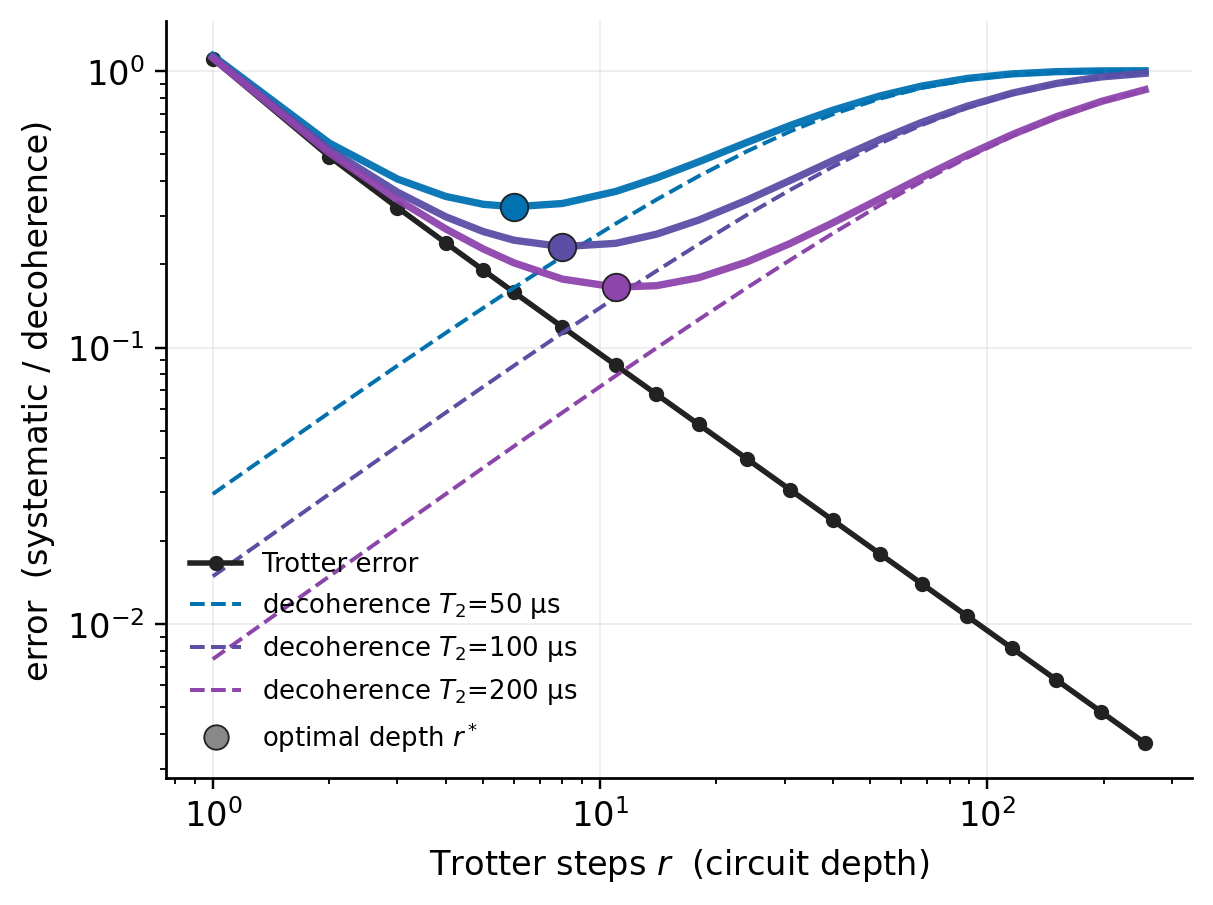
\includegraphics[width=\linewidth]{figs/prop_fig_coherence.png}\\[-2pt]
  {\footnotesize\textbf{(a)} coherence budget}
\end{minipage}\hfill
\begin{minipage}[t]{0.40\textwidth}\centering
  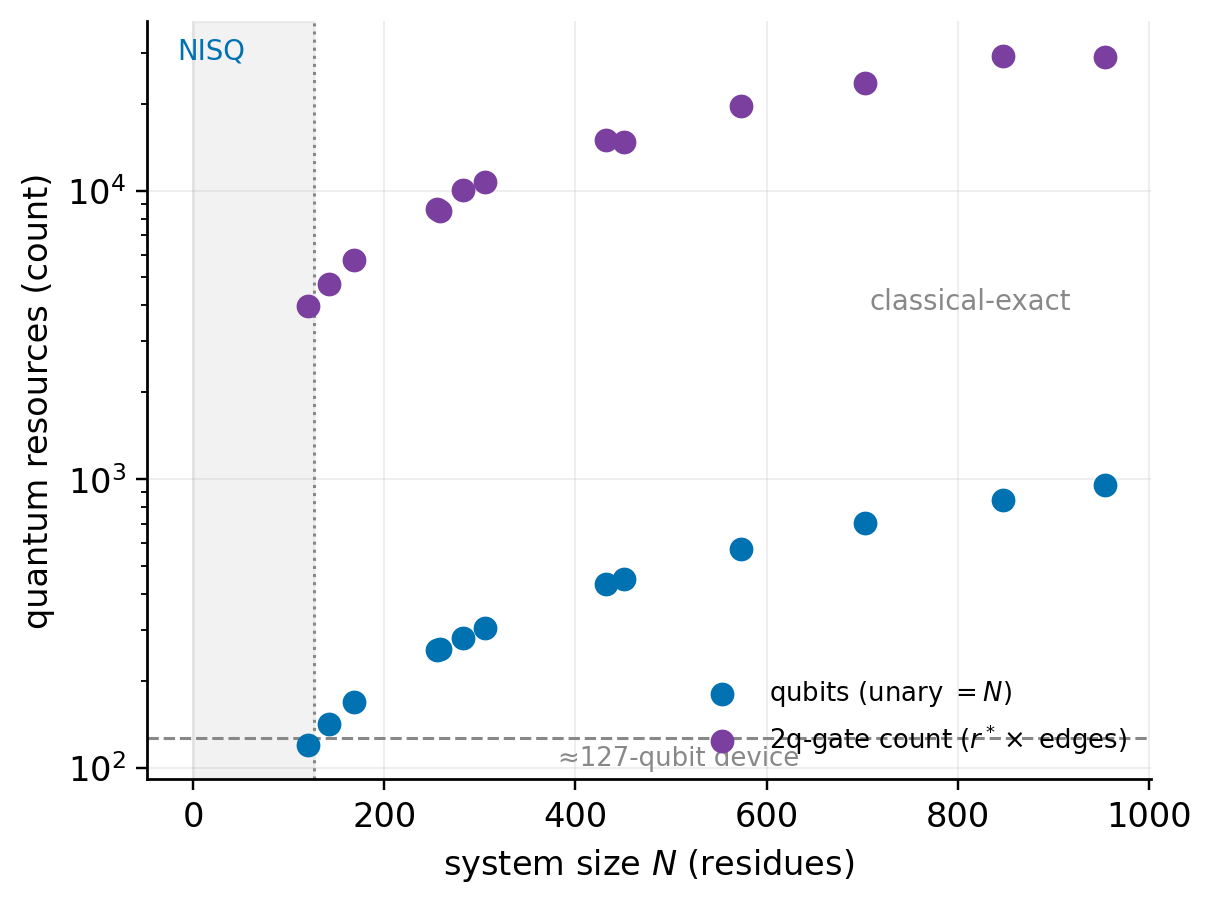
\includegraphics[width=\linewidth]{figs/prop_fig_resource.png}\\[-2pt]
  {\footnotesize\textbf{(b)} resource scaling}
\end{minipage}
\caption{Coherence-time limitation on the current model. \textbf{(a)} Trotter error falls with depth
$r$ while decoherence rises; their sum is minimised at an optimal depth $r^{*}\propto\sqrt{T_2}$, and
the ranking converges well inside $r^{*}$. \textbf{(b)} Unary qubits equal residue count and 2q-gate
count scales with contact edges: small targets are near-term-demonstrable, larger ones use the exact
classical track.}
\label{fig:budget}
\end{figure}

\lead{Reading the coherence budget.} Two errors must be separated (Fig.~\ref{fig:budget}a). The
systematic Trotter error falls with depth; decoherence rises with it; their sum sets an optimal depth
$r^{*}\propto\sqrt{T_2}$. What makes the method feasible is that the \emph{ranking} converges at a
depth well below $r^{*}$, so the walk is read before it decoheres. The binding constraint is
accumulated gate error rather than duration, which fixes the headline run at the smallest $K$ and the
smallest Trotter number passing a simulator convergence test and declares the large-$K$ circuits
simulator-only. Post-selection on excitation number turns much of the residual error into discarded
shots rather than biased estimates, making it the primary mitigation and ZNE the secondary one.

\lead{Readout, platform and budget.} Sampling a few evolution times gives the source row of $J$
directly, since the excited qubit labels the Krylov basis vector; results project back to residues by
$Q$. A one-dimensional chain needs no all-to-all connectivity, so superconducting devices on Braket
(IQM, Rigetti) are the economic fit, and Classiq supplies depth-constrained synthesis under a fixed
coherence budget. A full campaign --- simulator validation, noise modelling, a headline run with
zero-noise extrapolation and a cross-platform check --- is on the order of a minute of QPU time,
dominated by queueing and classical processing.

% =====================================================================
\section{Implementation Plan}

Phase~I delivers this specification; Phase~II builds and validates it. The circuit of Section~3.8 is
the defining construction; because its single-excitation sector is exactly solvable, the same directed
matrix $J$ is computed classically at full resolution, serving as both deliverable and hardware
reference, so no milestone depends on device availability.

\begin{enumerate}
\item \lead{Structure and features.} Fetch apo structures, select the catalytic domain, strip waters
      and heteroatoms, build the heavy-atom contact graph, and compute per-residue conservation.
\item \lead{Hamiltonian assembly.} Fuse contact magnitudes and the chiral phase (with the
      conservation diagonal as an ablation), z-score normalise, gauge-fix, assert Hermiticity.
\item \lead{Readout.} Exact matrix exponential to the directed current $J$, delivered as its
      time-averaged coherent form.
\item \lead{Ranking.} Compute $s$, $\rho$ and $z$; apply distal and neighbour filters; return the top
      five residues with optional pocket annotation.
\item \lead{Coherence sweep.} Lindblad dephasing scan from $p = 0$ to $p = 1$, reported against
      $e^{A}$ and $e^{-Lt}$.
\item \lead{Validation.} Blind runs on the four targets, then extended generalisation runs, against
      all baselines in Section~5.
\item \lead{Hardware.} Execute the circuits of Section~3.8 on Braket, verifying the quantum $J$
      against the classical one under post-selection and zero-noise extrapolation.
\end{enumerate}

\begin{table}[t]
\caption{Data and tools. No training set is required.}
\small
\begin{tabularx}{\textwidth}{@{}lX@{}}
\toprule
\textbf{Purpose} & \textbf{Source or tool}\\
\midrule
Required targets & RCSB PDB: 4OBE$\to$6OIM, 1OPL$\to$5MO4, 5TBY$\to$6C1H, 1NKP (c-Myc)\\
Calibration set & ASD, AlloBench: deduplicated by UniProt, length-binned, fixed seed; disjoint from targets\\
Structure and features & BioPython, ProDy (contact graph, ANM modes), fair-esm (ESM-2 conservation)\\
Simulation and readout & NumPy / SciPy matrix exponential for $J$; QuTiP for the Lindblad sweep\\
Circuits and hardware & Qiskit, AWS Braket SDK, Classiq (synthesis, depth optimisation), Mitiq (ZNE)\\
Baselines and output & fpocket, NetworkX, ProDy GNM centrality; PyMOL and browser viewer; LLM brief\\
\bottomrule
\end{tabularx}
\end{table}

\lead{Data processing and calibration set.} Structures are reduced to a single chain, stripped of
waters and heteroatoms, and mapped to a C$\alpha$ contact graph; UniProt active-site annotations are
aligned to the resolved sequence. Ground truth is frozen by the challenge rule --- residues with a
heavy atom within $4.5$~\AA\ of an allosteric-ligand heavy atom in the superposed holo structure. The
calibration set is drawn from the pooled ASD and AlloBench allosteric entries, deduplicated by UniProt
and stratified into length bins under a fixed seed, giving ten proteins that span the size range and
are disjoint from the blind targets; thresholds are fixed on it by leave-one-protein-out. No labels
enter the predictor, so the set calibrates but does not train.

\lead{Deliverables.} (i) The $N\times N$ directed connectivity matrix $J$ at full residue resolution.
(ii) Ranked top-five allosteric residues per target by $z(j)$. (iii) This methodological report,
identifying the directed current as the quantum metric and its vanishing in the classical limit as
its link to biological signal transmission. (iv) An interactive 3D map colouring the protein by $z(j)$
with predicted site and propagation paths (PyMOL and browser), the chemist-facing artefact, with the
language-model brief.

\lead{Feasibility within a 3--4 month sprint.} Every core deliverable is on the classical-exact track,
which needs no quantum device, so the schedule carries no external dependency: the structure pipeline
and Hamiltonian assembly, then the directed-current readout and ranking, then the blind runs,
baselines and coherence sweep, leave the hardware demonstration as a bounded add-on at the end.
Compute is a single-workstation eigenproblem for $N\approx300$--$1000$; data is public PDB and open
allosteric annotations; the only external cost is a minute-scale Braket campaign. The main assumptions
--- elastic-network dynamics and a chiral phase from the lowest ANM mode --- are stated and ablated,
so the plan is bounded by analysis effort, not by unproven capability.

\lead{Team.} Two members cover the competencies the method draws on. \textbf{I-Shan Tsai}
(Mathematics, UC~San Diego; Qiskit Advocate and Vice President of Quantum Computing at UCSD) brings
the quantum side --- quantum algorithms for electronic structure, quantum machine learning and
fault-tolerant circuit compilation, with a preprint accepted to IEEE Quantum Week (QCE~2026),
fragment-based quantum molecular generation at Taiwan's NCHC, and quantum engineering at Vernus~AI.
\textbf{Yu-Hsin Chen} (Institute of Bioinformatics and Systems Biology, NYCU) brings protein dynamics
and drug design --- generative models with molecular dynamics for protein drug design (PLMs, MD, PPI),
multiscale simulation in the Biosystems Simulation Lab, an RBX1 E3-ligase binder via MD and pretrained
PLMs, a 2026 Y~Combinator BIO$\times$AI Hackathon AI-Scientist-track win, and Qiskit Global Summer
School 2026. Together they span the quantum-walk, elastic-network and drug-discovery expertise the
proposal requires; being training-free, the method needs no specialised ML-ops capacity and runs on
commodity compute.

% =====================================================================
\section{Validation Plan}

\begin{table}[t]
\caption{Blind validation targets. The apo structure is the sole input; holo defines ground truth
only after predictions are frozen.}
\small
\begin{tabularx}{\textwidth}{@{}lcclc@{}}
\toprule
\textbf{Target} & \textbf{Apo} & \textbf{Holo} & \textbf{Site to blind-predict} & \textbf{Ref.}\\
\midrule
KRAS G12C       & 4OBE & 6OIM & Cryptic Switch-II pocket (sotorasib)            & \cite{ostrem2013}\\
BCR-ABL1        & 1OPL & 5MO4 & Distal myristoyl pocket (asciminib)             & \cite{wylie2017}\\
Cardiac myosin  & 5TBY & 6C1H & Site stabilising the super-relaxed state        & \cite{anderson2018}\\
c-Myc           & 1NKP & ---  & Myc--Max interface; pocket annotation disabled  & ---\\
\bottomrule
\end{tabularx}
\end{table}

\lead{Ground truth and controls.} Positive labels come from the holo structure and are used only after predictions are frozen: after
superposition onto apo coordinates, residues with a heavy atom within $4.5$~\AA\ of an
allosteric-ligand heavy atom are labelled allosteric, with indices mapped back through the apo--holo
alignment. Two negative sets match the controls named in the challenge. Random background draws
surface residues excluding the active site, its first neighbours and the labelled site.
Non-functional pockets are fpocket pockets on the apo structure overlapping neither the active site
nor any annotated functional site, scored by the same $z(j)$. The second is the stricter test, since
it excludes the possibility that the method merely separates pocket-like from non-pocket-like
surface.

\lead{Metrics and statistical tests.} Per target we report residue-level ROC-AUC, top-5 and top-10 hit rate, enrichment at top-$k$, and the
minimum C$\alpha$ distance from each predicted residue to the true site centre. Significance is
tested against each negative set by Mann--Whitney $U$ and by a permutation test resampling residues
matched on solvent accessibility and distance from the active site, so a geometric confound cannot
produce a significant result on its own. We report $p$-values with rank-biserial effect sizes and
bootstrap intervals on ROC-AUC. A target passes when both tests reach $p<0.05$ after Holm correction
across targets and the true site appears in the top five.

\lead{Baselines and ablations.} Baselines run on the identical graph: communicability
$e^{A}$~\cite{estrada2008}, diffusion $e^{-Lt}$, GNM centrality, bond-to-bond propensity~\cite{amor2016}
as the strongest published method here, PocketMiner ($0.87$)~\cite{meller2023} as the learned
reference, and a random ranking. The two sharing our graph and generator are decisive: they separate
interference from graph structure. Ablations remove one component at a time --- conservation diagonal,
chiral phase, degree deconfounding, background standardisation, and the readout swapped for its
symmetric comparators --- each reported as a $\Delta$ROC-AUC.

\lead{Robustness.} Noise resilience is assessed on the metric, not only on the state: we sweep the
dephasing $p$, simulate gate-error and finite-coherence models on DM1, and report the Spearman
correlation between noisy and noiseless $z(j)$ with top-5 overlap --- what matters is whether the
ranking survives. Coarse-graining fidelity uses the same measures between full-resolution $J$ and its
Krylov reduction, complementing the exactness identity~(5) with where truncation begins to matter.

\lead{Blind protocol and reproducibility.} No parameters are fitted, so leakage is structurally
limited: ground-truth labels are computed in a module the predictor cannot import (enforced by unit
test), thresholds come from leave-one-protein-out on a disjoint calibration set, and code, seeds and
intermediate matrices are released as a public code repository accompanying the submission, so each
figure regenerates from a clean checkout.

% =====================================================================
\section{Impact, Metrics of Success and Risks}

\lead{Where the value sits.} The tool acts where a target is advanced or abandoned. A static structure
becomes a ranked surface map in minutes, and being training-free it applies immediately to targets
with no allosteric precedent --- the population supervised predictors serve worst.

\lead{Metrics of success.} Discrimination against the published $0.87$~\cite{meller2023};
interference gain over $e^{A}$ and $e^{-Lt}$ on the same graph; runtime per target; top-5 hit rate
and distance to the true site; and generalisation on untouched ASD targets.

\lead{Risks.} The directed current depends on the chiral phase, so a target whose functional motion is
poorly captured by the lowest ANM mode weakens the signal; the phase and time window are reported with
sensitivity sweeps. The conservation diagonal is the main exposure to the ab-initio-from-topology
requirement, which is why the working model is topology-and-phase only. The elastic-network assumption
is weakest for c-Myc, delivered nonetheless with pocket annotation disabled. Finally, coherence may
carry little signal on a target, flattening the sweep toward chance --- a controlled outcome on a
question the challenge itself raises, with the classical pipeline still a working deliverable.

% =====================================================================
\clearpage
{\small\textit{Supplementary material (references).}}\par\vspace{0.3em}
\setlength{\columnsep}{16pt}
\begin{multicols}{2}
\begin{thebibliography}{99}
\setlength{\itemsep}{2pt}\setlength{\parskip}{0pt}\selectfont

\bibitem{godsil2013} Godsil C. Average mixing of continuous quantum walks.
  \textit{J. Comb. Theory Ser. A} \textbf{120}, 1649--1662 (2013). arXiv:1103.2578

\bibitem{mohtashim2026} Mohtashim SI, Sajjan M, Kais S. Continuous-time quantum-walk centrality for
  protein residue interaction networks. \textit{J. Am. Chem. Soc.} \textbf{148}, 29206--29219 (2026).
  doi:10.1021/jacs.6c08053

\bibitem{amor2016} Amor BRC, Schaub MT, Yaliraki SN, Barahona M. Prediction of allosteric sites and
  mediating interactions through bond-to-bond propensities. \textit{Nat. Commun.} \textbf{7}, 12477
  (2016). doi:10.1038/ncomms12477

\bibitem{novo2015} Novo L, Chakraborty S, Mohseni M, Neven H, Omar Y. Systematic dimensionality
  reduction for quantum walks. \textit{Sci. Rep.} \textbf{5}, 13304 (2015). doi:10.1038/srep13304

\bibitem{whitfield2010} Whitfield JD, Rodr\'iguez-Rosario CA, Aspuru-Guzik A. Quantum stochastic
  walks. \textit{Phys. Rev. A} \textbf{81}, 022323 (2010). doi:10.1103/PhysRevA.81.022323

\bibitem{mohseni2008} Mohseni M, Rebentrost P, Lloyd S, Aspuru-Guzik A. Environment-assisted quantum
  walks in photosynthetic energy transfer. \textit{J. Chem. Phys.} \textbf{129}, 174106 (2008).
  doi:10.1063/1.3002335

\bibitem{rebentrost2009} Rebentrost P, Mohseni M, Kassal I, Lloyd S, Aspuru-Guzik A.
  Environment-assisted quantum transport. \textit{New J. Phys.} \textbf{11}, 033003 (2009).
  doi:10.1088/1367-2630/11/3/033003

\bibitem{estrada2008} Estrada E, Hatano N. Communicability in complex networks.
  \textit{Phys. Rev. E} \textbf{77}, 036111 (2008). doi:10.1103/PhysRevE.77.036111

\bibitem{lu2016} Lu D, Biamonte JD, Li J, et al. Chiral quantum walks. \textit{Phys. Rev. A}
  \textbf{93}, 042302 (2016). doi:10.1103/PhysRevA.93.042302

\bibitem{bahar1997} Bahar I, Atilgan AR, Erman B. Direct evaluation of thermal fluctuations in
  proteins using a single-parameter harmonic potential. \textit{Folding \& Design} \textbf{2},
  173--181 (1997). doi:10.1016/S1359-0278(97)00024-2

\bibitem{atilgan2001} Atilgan AR, Durell SR, Jernigan RL, et al. Anisotropy of fluctuation dynamics
  of proteins with an elastic network model. \textit{Biophys. J.} \textbf{80}, 505--515 (2001).
  doi:10.1016/S0006-3495(01)76033-X

\bibitem{chennubhotla2007} Chennubhotla C, Bahar I. Signal propagation in proteins and relation to
  equilibrium fluctuations. \textit{PLoS Comput. Biol.} \textbf{3}, 1716--1726 (2007).
  doi:10.1371/journal.pcbi.0030172

\bibitem{meller2023} Meller A, Ward M, Borowsky J, et al. Predicting locations of cryptic pockets
  from single protein structures using the PocketMiner graph neural network.
  \textit{Nat. Commun.} \textbf{14}, 1177 (2023). doi:10.1038/s41467-023-36699-3

\bibitem{asbench2015} Huang Z, et al. ASBench: benchmarking sets for allosteric discovery.
  \textit{Bioinformatics} \textbf{31}, 2357--2359 (2015). doi:10.1093/bioinformatics/btv169

\bibitem{ostrem2013} Ostrem JM, Peters U, Sos ML, Wells JA, Shokat KM. K-Ras(G12C) inhibitors
  allosterically control GTP affinity and effector interactions. \textit{Nature} \textbf{503},
  548--551 (2013). doi:10.1038/nature12796

\bibitem{wylie2017} Wylie AA, Schoepfer J, Jahnke W, et al. The allosteric inhibitor ABL001 enables
  dual targeting of BCR--ABL1. \textit{Nature} \textbf{543}, 733--737 (2017). doi:10.1038/nature21702

\bibitem{anderson2018} Anderson RL, Trivedi DV, Sarkar SS, et al. Deciphering the super relaxed state
  of human $\beta$-cardiac myosin and the mode of action of mavacamten. \textit{PNAS} \textbf{115},
  E8143--E8152 (2018). doi:10.1073/pnas.1809540115

\end{thebibliography}
\end{multicols}

\end{document}
